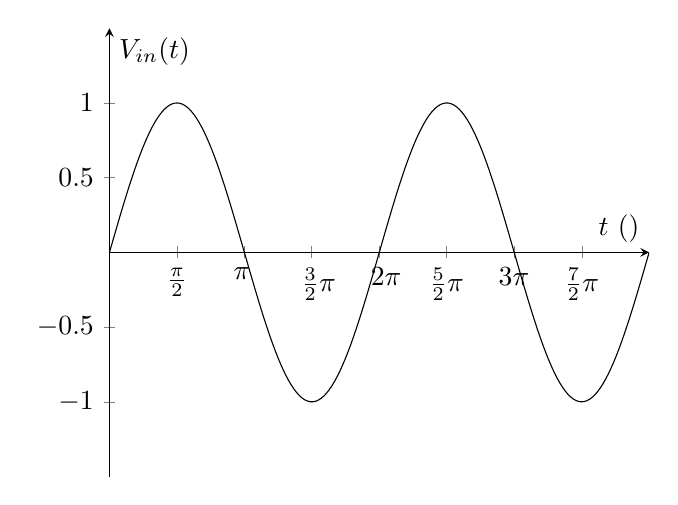
\begin{tikzpicture}
\begin{axis}[
    axis lines = middle,
    xlabel = {$t$ $(\si{\milli\second})$},
    ylabel = {$V_\text{in}(t)$},
    xtick={0,1.57,3.14,4.71,6.28, 7.85, 9.42, 11.00, 12.57},
    xticklabels={$0$, $\frac{\pi}{2}$,$\pi\,$,$\,\,\,\frac{3}{2}\pi$,$\,\,\,2\pi$, $\frac{5}{2}\pi$, $3\pi$, $\frac{7}{2}\pi$, $4\pi$},
    ytick={0,-0.5,0.5,-1,1},
    ymin=-1.5,
    ymax=1.5,
    xmin = 0,
    xmax=4*pi
]
\addplot [
	color=black,
	domain=0:4*pi,
	samples=200
	]
	{ sin(deg(x))  
	};
\end{axis}
\end{tikzpicture}